\section{Modulação Digital}
\label{sec:bpsk}

A modulação BPSK é uma modulação por deslocamento de fase onde, dado um sinal digital, cada zero ou um são associados a mudanças na fase do sinal da portadora, porém, a fase continua a mesma.
BPSK também é conhecida como 2-PSK, pois utiliza apenas duas fases para representar as variações no sinal digital, e.g. zeros recebem fase $\pi \textrm{ rad}$ e uns recebem $0 \textrm{ rad}$, vide figura~\ref{fig:bpskplot}.

\begin{figure}[H]
    \centering
    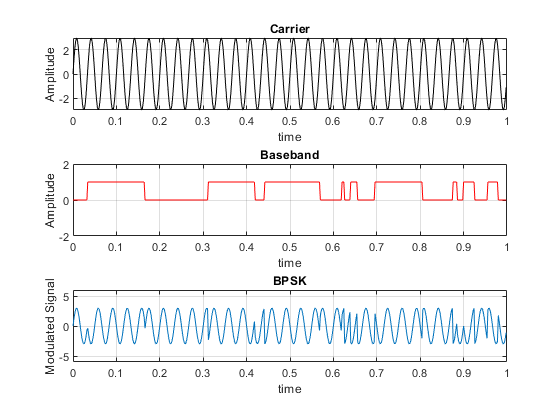
\includegraphics[width=0.65\textwidth]{figures/bpskplot.png}
    \caption{Gráficos de representação da modulação BPSK}
    \label{fig:bpskplot}
\end{figure}